\documentclass[tikz,border=4pt]{standalone}
\usepackage{pgfplots}
\pgfplotsset{compat=1.16}
% un colore per ogni Q, gli stessi in tutti i diagrammi del secondo ordine
\colorlet{Q05}{green!50!black}     % Q = 0,5
\colorlet{Q0707}{blue}             % Q = 0,707 (Butterworth)
\colorlet{Q1}{orange}              % Q = 1
\colorlet{Q2}{magenta}             % Q = 2
\colorlet{Q5}{black}               % Q = 5
\pgfplotsset{
  bode/.style={
    width=6.4cm, height=4.4cm, xmin=0.01, xmax=100,
    grid=both, major grid style={gray!55}, minor grid style={gray!20},
    tick label style={font=\footnotesize}, label style={font=\small},
    title style={font=\small}, xlabel={$\omega/\omega_u$},
  },
  bode mag/.style={bode, ymin=-50, ymax=50, ytick={-40,-20,0,20,40},
    ylabel={$|H|_{\mathrm{dB}}$}, title={Modulo}},
  bode fase/.style={bode, ymin=-100, ymax=100, ytick={-90,-45,0,45,90},
    ylabel={$\varphi$ [$^\circ$]}, title={Fase}},
}
\begin{document}
% Sallen-Key passa-alto, K = 1:  H(j w) = -x^2 / ((1-x^2) + j x/Q),  x = w/w0
% |H|_dB = 40 log x - 10 log[(1-x^2)^2 + x^2/Q^2],   fase = 180 - atan2(x/Q, 1-x^2)
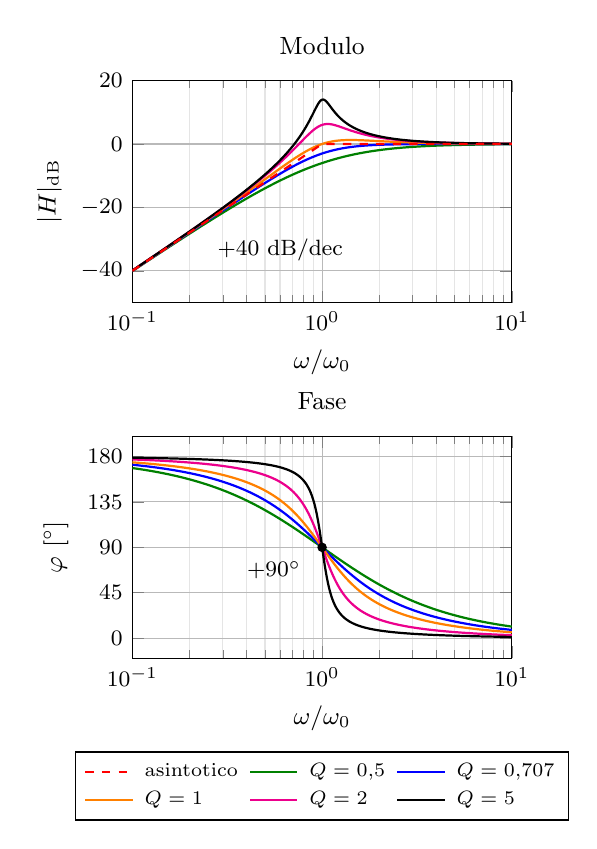
\begin{tikzpicture}
% ---------- modulo ----------
\begin{semilogxaxis}[bode mag, name=mag, xmin=0.1, xmax=10, xlabel={$\omega/\omega_0$},
  ymin=-50, ymax=20, ytick={-40,-20,0,20}]
  \addplot[Q05, thick, domain=-1:1, samples=301]
    ({10^x}, {40*x - 10*log10((1-10^(2*x))^2 + (10^x/0.5)^2)});
  \addplot[Q0707, thick, domain=-1:1, samples=301]
    ({10^x}, {40*x - 10*log10((1-10^(2*x))^2 + (10^x/0.7071)^2)});
  \addplot[Q1, thick, domain=-1:1, samples=301]
    ({10^x}, {40*x - 10*log10((1-10^(2*x))^2 + (10^x/1)^2)});
  \addplot[Q2, thick, domain=-1:1, samples=301]
    ({10^x}, {40*x - 10*log10((1-10^(2*x))^2 + (10^x/2)^2)});
  \addplot[Q5, thick, domain=-1:1, samples=301]
    ({10^x}, {40*x - 10*log10((1-10^(2*x))^2 + (10^x/5)^2)});
  \addplot[red, thick, dashed] coordinates {(0.1,-40) (1,0) (10,0)};
  \node[anchor=north west, font=\footnotesize] at (axis cs:0.25,-27) {$+40$ dB/dec};
\end{semilogxaxis}
% ---------- fase ----------
\begin{semilogxaxis}[bode fase, at={(mag.south west)}, yshift=-1.7cm, anchor=north west,
  xmin=0.1, xmax=10, xlabel={$\omega/\omega_0$},
  ymin=-20, ymax=200, ytick={0,45,90,135,180},
  legend columns=3, legend style={font=\scriptsize, at={(0.5,-0.42)}, anchor=north, column sep=2pt},
  legend cell align=left]
  \addlegendimage{red, thick, dashed}
  \addlegendentry{asintotico}
  \addplot[Q05, thick, domain=-1:1, samples=301]
    ({10^x}, {180-atan2(10^x/0.5, 1-10^(2*x))});
  \addlegendentry{$Q=0{,}5$}
  \addplot[Q0707, thick, domain=-1:1, samples=301]
    ({10^x}, {180-atan2(10^x/0.7071, 1-10^(2*x))});
  \addlegendentry{$Q=0{,}707$}
  \addplot[Q1, thick, domain=-1:1, samples=301]
    ({10^x}, {180-atan2(10^x/1, 1-10^(2*x))});
  \addlegendentry{$Q=1$}
  \addplot[Q2, thick, domain=-1:1, samples=301]
    ({10^x}, {180-atan2(10^x/2, 1-10^(2*x))});
  \addlegendentry{$Q=2$}
  \addplot[Q5, thick, domain=-1:1, samples=301]
    ({10^x}, {180-atan2(10^x/5, 1-10^(2*x))});
  \addlegendentry{$Q=5$}
  \addplot[only marks, mark=*, mark size=1.5pt, black] coordinates {(1,90)};
  \node[anchor=north east, font=\footnotesize] at (axis cs:0.87,86) {$+90^\circ$};
\end{semilogxaxis}
\end{tikzpicture}
\end{document}
